\begin{center}
  \section{Limits, nets and homeomorphisms}
\end{center}

\setcounter{section}{2}
\begin{qst}[A classical counterexample of non-Hausdorff space]
Let $R^* = \mathbb R \setminus \set{0}$ and $E = R^* \cup \set{-\infty,+\infty}$. A set $A \subseteq E$ is open if it satisfies
\begin{enumerate}[i.]
  \item $A \cap R^*$ is open in the topological space $R^*$ endowed with the usual topology, and 
  \item if $+\infty \in A$ or $-\infty \in A$, then $A$ includes some set   $R^* \cap U$ where $U$ is a neighborhood of $0$ in $\mathbb R$.
\end{enumerate}
Show that:
\begin{enumerate}[(a)]
  \item The collection of sets that satisfy conditions (i) and (ii) constitute a topology. Denote the topological space by $(E,\tau)$.
  \item The topological space $(E,\tau)$ is non-Hausdorff.
  \item The intersection of all neighborhoods of $x \in E$ is $\set{x}$. That is,
     $\bigcap_{V \in \cN(x)} V = \{x\}$ for all $x \in E$. [Hint: What are the closed sets in $E$?] 
\end{enumerate}  
\end{qst}


\subsection{The closure and the interior}

Denote by $E$ a topological space and let $A \subset E$. 
A point $x \in E$ is called an
\textit{adherent point}\footnote{Also known as closure point or contact point.}
of set $A$ if every neighborhood of $x$  
contains at least one point of $A$.
In addition, if every neighborhood of $x$  
contains at least one point of $A$ different from $x$, 
it is called a \textit{limit point} of set $A$. 

\begin{qst}
  Denote by $\bar A$ the set of all adherent points of $A$.
\begin{enumerate}[(a)]
  \item Show that $\bar A$ is closed.
  \item Show that $A \subseteq \bar A$.
  \item Show that $\bar A$ is the smallest closed set that contains $A$. [For that reason, $\bar A$ is also called the closure of $A$.]
\end{enumerate} 
\end{qst}

\begin{asw}
  
\end{asw}


A point $x \in E$ is called an interior point of $A$ if there exists a neighborhood $U$ of $x$ such that $U \subseteq A$.
Denote by $\mathring A$ the set of its interior points.
Formally $\mathring A$ is known as the interior of set $A$.

\begin{qst}
  \begin{enumerate}[(a)]
    \item Show that $\mathring A \subset A$.
    \item Show that $\mathring A$ is open. 
    \item Show that $\mathring A$ is the largest open set included in $A$.
    \item Show that $A$ is open if and only if $\mathring A = A$.   
  \end{enumerate} 
\end{qst} 

\begin{asw}
  
\end{asw}

The following are useful properties of the closure and interior of set $A$. Proving them is also an incredible chance to review the language of basic topology (e.g.\ open and closed sets, neighborhoods, and the set operations on them....) 

\begin{qst}
  \begin{enumerate}[(a)]
    \item Show that $\mathring{A}=\mathring{\mathring{A}}$ and $\bar A = \bar{\bar{A}}$.
    \item Show that $E \setminus \mathring A = \overline{E \setminus A}.$
    \item Show that $\bar A \cup \bar B = \overline{A \cup B}$ and 
      $\mathring A \cap \mathring B = \mathring{\widehat{A \cap B}}$ where 
      $\mathring{\widehat{A \cap B}}$ is the interior of the intersection of $A$ and $B$. 
  \end{enumerate} 
\end{qst} 

\subsection{Limits of a  sequence v.s.\ limit points of a set}

Given a sequence $(x_n)_{n \in \mathbb N}$ in $(E, \tau)$,
we say $x \in E$ is a \textit{limit} of $(x_n)$ if for any neighborhood $V$ of $x$, there exists some $N$ such that $x_n \in V$ for all $n>N$.
A sequence $(x_n)$ need not have a limit; and when it has, it can have multiple limits.
We say $(x_n)$ in $(E, \tau)$ is \textit{convergent} if it approaches some limit $x \in E$, formally written as $\tau \text{-} \lim_{n\to\infty} x_n = x$. We use the shorthand $\lim_{n\to\infty} x_n$ (i.e.\ dropping the $\tau$ beforehand)  when there's no ambiguity.

\begin{qst}
  Let $E = \set{a,b,c}$ endowed with a topology 
  $$\tau = \big\{ \set{a,b},\set{b,c}, \set{b}, E, \emptyset \big\},$$
  \begin{enumerate}[(a)]
    \item What are the limit points (if any) of $(x_n)$ where $x_n = b$ for each $n$? 
    \item Is $(E,\tau)$ a Hausdorff space?
    \item Show that if $(E,\tau)$ is a topological space, then any convergent sequence in $E$ has a unique limit.
  \end{enumerate}
\end{qst}

\medskip

You may wonder whether we can use the \textit{limits of each sequence} $(x_n)$ in $A \subseteq E$ to get the \textit{limit points of} $E$.
However, this does not hold in a general topological space.

\begin{qst}[cocountable topology] 
Let $E = R$ and call a set $A \subseteq E$ open if $A^c$ is countable.
\begin{enumerate}[(a)]
  \item Show that the set of ``open sets'' defined above constitute a topology. 
   
  Denote the topology by $\tau$.
  
  \item Show that in $(E, \tau)$ a sequence $(x_n)$ is convergent if and only if $x_n$ is a constant after some $x_N$. 
  \item Illustrate that there exists some set $A \subset E$ whose limit points cannot be approached by any sequence in $A$.
\end{enumerate}  
\end{qst}

\subsection{Nets}


Plain sequences detect topological properties in metric spaces, but they fail to do so in more general topological spaces.
That motivates the concept of \textit{nets}.\footnote{A great introduction to nets can be found at nLab: \url{https://ncatlab.org/nlab/show/net}.}
A net is a function $\nu$ from a special preordered set $D$ to the topological set $E$.


\noindent \textbf{Definition [Directed set].}
A \textit{directed set} is a preordered set $(D, \le)$
\footnote{Here $D$ is equipped with a reflexive and transitive relation. For a  concrete example, think of $\le$ as the preference relation.}
such that every finite subset has an upper bound. That is,  for any
$a,b \in D$ there exists $c \in D$ 
such that $a \le c$ and $b \le c$.

Examples of directed sets include 
a directed set of natural numbers and a directed set of neighborhoods.
Specifically, let $A_{\ge}$ and  $B_{\ge}$ be directed sets.
Then the Cartesian product $A \times B$ of the underlying sets becomes itself a directed set by setting
$$
(a_1, b_1) \leq (a_2, b_2) \text{ if } a_1 \le a_2, b_1 \le b_2
$$


\noindent \textbf{Definition [Nets].}
A net in a set $X$ is
\begin{enumerate}
  \item  a directed set $A$, called the index set, and
  \item  a function $\nu \colon A \to X$, from the underlying set $A$ to $X$.
\end{enumerate}
We say $\nu$ is a net and set $A$ indexes the net.
For example, a sequence is a net whose directed set of indices is the natural numbers. 
Since $A$ is a preordered set, it makes sense to talk like ``For any neighborhood $U$ of $x$, there exists $i \in A$ such that for all $j \ge i$ we have $v_j \in U$.''
A directed set $A$ is a natural extension of $\mathbb N$, 
and we use $A$ rather than $\mathbb N$ to index a set.


Consider net $\nu: A \to X$ and given a subset $S \subset X$. We say that\footnote{Sometimes one says `infinitely often' in place of `frequently' and even `cofinitely often' in place of `eventually.'
These derive from the special case of sequences, where they may be taken literally.}
\begin{enumerate}
  \item $\nu$ is \textit{eventually} in $S$ if there exists $i \in A$ such that $\nu_j \in S$ for each $j \ge i$.
  \item $\nu$ is \textit{frequently} in $S$ if for every index    $i \in A$ there exists some $j \ge i$ such that $\nu_j \in S$.
\end{enumerate}

I will not go into the details here. Instead, I urge you to read the exposition of nets at nLab.
A beautiful result is that a topological space $(E,\tau)$ is compact if and only if every net in $X$ has a sub-net that converges.


\subsection{Continuous mappings and homeomorphisms}

Given two topological spaces $E$ and $F$ and a mapping $f: E \to Y$, let $x \in E$ and denote its image by $f(x)$.
We say $f$ is continuous at $x \in E$ if for any neighborhood $V$ of $f(x)$, 
the inverse image of $V$, $f^{-1}(V)$ is a neighborhood of $x$.
We say $f$ is continuous on $E$ if it is continuous at each $x \in E$.

If you do not like the usage of neighborhoods and prefer using open sets, 
an equivalent definition is that $f \colon E \to F$ is open on $E$ 
if $f \inv (O)$ is open for each open set $O \subseteq F$.
You are asked to prove that in Question \ref{qst:conti}.

\begin{qst} \label{qst:conti}
  Let $E$ and $F$ be two topological spaces and $f: E\to F$ be a mapping from $E$ to $F$. Show that the following statements are equivalent:
  \begin{enumerate}
    \item $f$ is continuous on $E$
    \item $f \inv (O)$ is open for each open set $O \subseteq F$
    \item $f \inv (A)$ is closed for each closed set $A \subseteq F$ 
  \end{enumerate}
\end{qst} 

Continuous mappings are nice animals. The composition of two continuous mappings is still continuous.
As the continuity of $f$ depends on the topologies on $E$ and $F$,
you can trick your calculus teacher by claiming that every real function is continuous! As long as you equip $R$ with the strongest topology --- discrete topology.


Given two topological spaces $E$ and $F$, we say they are \textit{homeomorphic}
if there exists some bijection $f: E \to F$ such that both $f$ and
$f \inv$ are continuous. We call such $f$ a \textit{homeomorphism}  between the two topological spaces $E$ and $F$.

Homeomorphism is the `isomorphism' between topological spaces.
Two homeomorphic topological spaces are basically the same for the purposes of topology.
A left and right glove are identical, because the left-right reflection is continuous in both directions. The difference between the left and right gloves isn't intrinsic to the gloves themselves, but is in the way the gloves are embedded in three-dimensional space.
Another classic example is the
cup--donut topological equivalence. 
Imagine continuous mappings as deformations of elastic physical bodies, which may be deformed by stretching them without tearing.
By doing that, you can turn a coffee cup to a donut (or formally, a torus). 

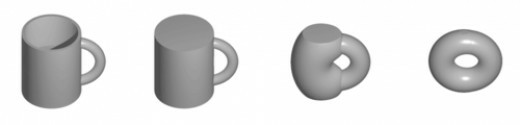
\includegraphics[width=\textwidth]{cup.jpg}

\begin{qst} Consider $\mathbb R$ endowed with the usual topology.
  \begin{enumerate}[(a)]
    \item Prove that any open interval $(a,b)$ is homeomorphic to the interval $(0,1)$. Here both $a$ and $b$ can be infinite. 
    \item Prove that any two bounded closed intervals of the real line are homeomorphic; i.e., $[a,b]$ is homeomorphic to $[0,1]$.  
    \item Show that if we drop out `bounded,' the statement above does not hold. [Hint: compactness]
  \end{enumerate}
\end{qst}



\subsubsection{From homeomorphism to knot theory}

I cannot help but talk more about these embedding stuff.
Consider this analogy: The symbol \texttt{b} can be turned into \texttt{d}, 
but to do it you have to lift the b out of the plane and flip it over. If you leave b and d embedded in the plane you can never turn one into the other (although you can turn b into q and d into p). 
So the difference is not in the shapes \textit{themselves}
but in the way they inhabit the plane.
Left and right gloves are distinguishable if they remain in three-dimensional space.
But in larger spaces, they're identical. It's easy to turn a left glove into a right glove if you can lift it into four-dimensional space and flip it over.

The branch of topology called ``knot theory'' concerns the way simple shapes like circles can be embedded into three dimensions.
Topologically a knotted loop of string and an unknotted one are the same --- but again, their embeddings into three-dimensional space are different. 

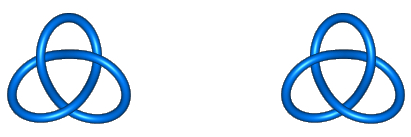
\includegraphics[width=0.8\textwidth]{knots}


Dealing with this topologically requires extra efforts.
One embeds the knotted loop in space and then considers whether there is a continuous deformation of the entire space, including the loop, that transforms the knotted loop into the unknotted one. Viewed in this way one can say that a trefoil knot (shown in the image) is chiral, 
because although each is topologically equivalent to a plain circle, the left-handed trefoil knot can never be smoothly transformed into the right-handed one
without removing it from three-dimensional space.

So next time do not leave a bad review when you receive a pair of left-hand gloves. They are actually the same with right-hand gloves! 
After all, according to some really smart physicists the universe we inhabit is made of 11 dimensions.


\begin{qst}
  Consider the coffee mug and torus example. Is the coffee mug shown in the image
  chiral? How about the torus?
\end{qst}

\begin{asw}
  A coffee mug is \textit{not} chiral in the topological sense. 
  It has a handle on the left side, and we can deform space to move the handle to the right side instead: just turn the cup around, now the handle is on the other side. No fourth dimension is required. 
  There are also many other ways to get the handle to the other side.
\end{asw}

\begin{qst}[Just for fun]
  Is a ball (sphere + interior) being equivalent to a (solid) cube? 
  A topologist answers yes and an algebraist answers no. Explain the differences.
\end{qst}

\begin{asw}
  Topology is ``geometry minus shape.'' That is, we topologists are completely ignoring the exact shape of an object.   Topological equivalence only cares about preserving a special closeness relation (i.e.\ homeomorphism) between the points of an object.
  So a ball is equivalent to a cube.

  They algebraists care about the group of symmetries.
  The sphere having infinitely many symmetries, while a cube only has a finite symmetry group.
\end{asw}


